\documentclass[a4paper]{ltjsbook}
%\usepackage{titlepage}

%theobibliographyのタイトルを変更
\renewcommand{\bibname}{参考文献}

\newcommand{\R}{\mathbb{R}} %実数の集合
\newcommand{\C}{\mathbb{C}} %虚数の集合
\newcommand{\N}{\mathbb{N}} %自然数の集合
\newcommand{\Q}{\mathbb{Q}} %有理数の集合
\newcommand{\Z}{\mathbb{Z}} %整数の集合
\newcommand{\Prob}{\mathbb{P}} %確率
\newcommand{\E}{\mathbb{E}} %期待値
\newcommand{\Var}{\text{Var}} %分散
\newcommand{\Cov}{\text{Cov}} %共分散
\newcommand{\delt}{\Delta t}%時刻の微小変化
%使用するパッケージをまとめておく
\usepackage{bm}
\usepackage{amsmath,amssymb,amsthm,thmtools,mathtools,latexsym}
\usepackage{listings,jvlisting}
\renewcommand{\lstlistingname}{ソースコード} %ここに挿入してないとダメ
\usepackage[margin=20truemm]{geometry}
%ここからソースコードの表示に関する設定
\lstset{
    basicstyle={\ttfamily},
    identifierstyle={\small},
    commentstyle={\smallitshape},
    keywordstyle={\small\ttfamily},
    frame={tb},
    breaklines=true,
    columns=[l]{fullflexible},
    numbers=left,
    %xrightmargin=0zw,
    %xrightmargin=1.6zw,
}
\pagestyle{plain}
\begin{document}
%タイトルベージを作成
\begin{titlepage}
\Large
\begin{center}
\vspace*{80pt}aligned
    {\huge 日本語タイトル} \\
\vspace*{10mm}
    {\huge english title}
\vspace*{80mm} \\
合田 理樹

\vspace*{10mm}
\begin{tabular}{ll}
    指導教員 & 降籏 大介 \\
    副指導教員 & 宮武 勇登 \\
\end{tabular}
\vspace*{20mm} \\
令和7年2月 \\
\end{center}
\end{titlepage}

%目次
\tableofcontents

%序論
\chapter{序論}
\section{研究背景}
$\bm{R}$
\section{研究目的}
A \\
s \\
x\\
xx\\
cc \\
cc\\
v\\
v\\
vv\\
f\\
f\\
\section{本論文の構成}
dd\\
cc \\
d\\
dd\\
cc\\
cc\\
hh\\
nnn\\
nn\\
ff\\
bbb\\
bbbb\\
mmm\\

%〇〇についての基礎知識
\chapter{浮動小数点数と固定小数点数についての基礎知識}
\label{chap:基礎知識1}
計算機内部で扱う数値には二つの表現方法がある.
それぞれの表現方法を固定小数点数がと浮動小数点数という.これらの表現方法について説明する.
固定小数点数,浮動小数点数はともに数を計算機が記憶しておくための数の表現方法である.

\section{固定小数点}
固定小数点数は,与えられたbit数に対して,そのうち小数部にいくつのbitを割り当てるのかを決めて残りのbitを整数部に割り当てて数を表現する方法である.
例として,$N \in \N$として計算機の中で$N$bitが数字を記憶するために与えられているとする.
そのうち,$m \ (m < N)$bitを小数部に割り当てた固定小数点数$a$は,符号を考えない場合以下のように表すことができる:

\begin{align}
    a = a_{N-m-1} 2^{N-m-1} + a_{N-m-2} 2^{N-m-2} + \cdots + a_1 2^1 + a_0 2^0 + a_{-1} 2^{-1} + \cdots + a_{-m} 2^{-m}.
\end{align}
ただし,$a_{i} \ (i = N-m-1,N-m-2,\dots,1,0,-1,\dots,-m)$は$0$または$1$の値を取る.
\begin{figure}[H]
    \centering
    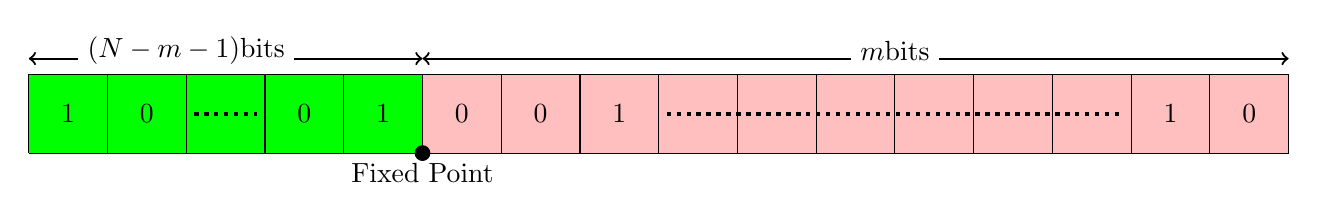
\begin{tikzpicture}
        \fill[green] (0,0) rectangle (5,1);
        \fill[pink] (5,0) rectangle (16,1);
        \draw (0,0) grid (16,1);
        \fill (5,0) circle [radius=0.1] node [below] {Fixed Point};
        \draw[ultra thick, dotted] (2.1,0.5) -- (2.9,0.5);
        \node [anchor=center] at (0.5,0.5) {1};
        \node [anchor=center] at (1.5,0.5) {0};
        \node [anchor=center] at (3.5,0.5) {0};
        \node [anchor=center] at (4.5,0.5) {1};
        \node [anchor=center] at (5.5,0.5) {0};
        \node [anchor=center] at (6.5,0.5) {0};
        \node [anchor=center] at (7.5,0.5) {1};
        \draw[ultra thick, dotted] (8.1,0.5) -- (13.9,0.5);
        \node [anchor=center] at (14.5,0.5) {1};
        \node [anchor=center] at (15.5,0.5) {0};
        \draw[<->,thick] (0,1.2) -- (5,1.2);
        \draw (2,1.3) node[fill=white] {$(N-m-1)$bits};
        \draw[<->,thick] (5,1.2) -- (16,1.2);
        \draw (11,1.3) node[fill=white] {$m$bits};
    \end{tikzpicture}
    \caption{$N$bitの符号なし固定小数点のイメージ図}
    \label{fig:fixedpointnumber_unsigned}
\end{figure}
また,符号付き固定小数点の場合,符号に$1$bit割り当てるため整数部が$N-m-2$bitとなる.
\begin{figure}[H]
    \centering
    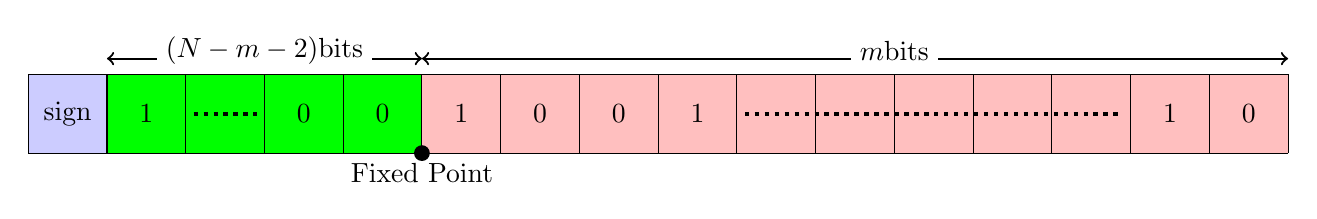
\begin{tikzpicture}
        \fill[green] (1,0) rectangle (5,1);
        \fill[pink] (5,0) rectangle (16,1);
        \fill[blue, opacity=0.2] (0,0) rectangle (1,1);
        \draw (0,0) grid (16,1);
        \fill (5,0) circle [radius=0.1] node [below] {Fixed Point};
        \draw[ultra thick, dotted] (2.1,0.5) -- (2.9,0.5);
        \node [anchor=center] at (0.5,0.5) {sign};
        \node [anchor=center] at (1.5,0.5) {1};
        \node [anchor=center] at (3.5,0.5) {0};
        \node [anchor=center] at (4.5,0.5) {0};
        \node [anchor=center] at (5.5,0.5) {1};
        \node [anchor=center] at (6.5,0.5) {0};
        \node [anchor=center] at (7.5,0.5) {0};
        \node [anchor=center] at (8.5,0.5) {1};
        \draw[ultra thick, dotted] (9.1,0.5) -- (13.9,0.5);
        \node [anchor=center] at (14.5,0.5) {1};
        \node [anchor=center] at (15.5,0.5) {0};
        \draw[<->,thick] (1,1.2) -- (5,1.2);
        \draw[<->,thick] (5,1.2) -- (16,1.2);
        \draw (3,1.3) node[fill=white] {$(N-m-2)$bits};
        \draw (11,1.3) node[fill=white] {$m$bits};
    \end{tikzpicture}
    \caption{$N$bitの符号付き固定小数点のイメージ図}
    \label{fig:fixedpointnumber_signed}
\end{figure}
本論文では,$N$bitの符号付き固定小数点で小数部に$m$bit,整数部に$(N-m-2)$bitを割り当てた固定小数点を,
\begin{equation}
    \text{Q}(N-m-2)\text{f}m
\end{equation}
と表す.
例えば,Q11f52は符号に1bit,小数部に52bit,整数部に11bitを割り当てた固定小数点数のことを表す.
\section{浮動小数点}
浮動小数点は,与えられたbit数に対して,bitを仮数部と指数部にわけて数を表現する方法である.
仮数部の数を$m$,指数部の数を$e$とすると浮動小数点$b$は,以下の様に表現することができる:
\begin{align}
    b = m \times 2^e.
\end{align}
ここで$m,e$はともに2進数の数である.
浮動小数点については,国際的な規格があり,割り当てられるbit数が32bit,64bitのものをそれぞれ単精度浮動小数点(Float32),倍精度浮動小数点(Float64)という.
それぞれの浮動小数点数の仮数部と指数部のbit数は以下の表のように決められている:
\begin{table}[H]
    \centering
    \caption{単精度浮動小数点(Float32)と倍精度浮動小数点(Float64)の仮数部と指数部のbit数}
    \begin{tabular}{c|c|c}   
     & 仮数部 & 指数部 \\ \hline
    Float32 & 23bit & 8bit \\ 
    Float64 & 52bit & 11bit
    \end{tabular}
    \label{tab:Float32_Float64_bit}
\end{table}
浮動小数点はbit数によって表現出来る数の範囲が異なる.
単精度浮動小数点と倍精度浮動小数点では以下の様になる:
\begin{table}[H]
    \centering
    \caption{単精度浮動小数点と倍精度浮動小数点の表現可能な数の範囲}
    \begin{tabular}{c|c|c|c}   
     & 最大値 & 最小値 & 0に最も近い数 \\ \hline
    Float32 & & & \\
    Float64 & & &
    \end{tabular}
    \label{tab:Float32_Float64_range}
\end{table}

%まるまるについての基礎知識2
\chapter{丸め誤差・情報落ち・桁落ちについての基礎知識}
前章で述べたように計算機の中では表現できる数に限りがある.
そのため計算機の中で表現できる数はそのままの数で計算を行うが,計算機の中で表現できない数はその数にできるだけ近い表現をできる数を代わりに用いて計算を行うことになる.
ある数$a\ \in \R$に対して,計算機で$a$という数を扱う場合の表現を
\begin{equation}    
    a^{\ast} \ (\in \mathbb{F})
\end{equation}
とする.
また,$a$を$p$進数で表現することを明記する場合,
\begin{equation}
    a_{(p)}
\end{equation}
と表すことにする.
\label{chap:基礎知識2}
\section{丸め誤差}
丸め誤差について説明する.
丸め誤差とは,計算機を用いて数を計算する際に用いる誤差である.
真の値を$x_{\mathrm{true}} \ (\in \R)$とする.
計算機の中で表現できる数で$x_{\mathrm{true}}$に一番近い数を$x^{\ast} \ (\in \mathbb{F})$とすると,そのときの丸め誤差$e_{round}$は,
\begin{equation}
    e_{\mathrm{round}} = x_{\mathrm{true}} - x^{\ast}
\end{equation}
と表せる.
簡単のため,計算機で扱われる2進数ではなく10進数を用いた場合を考える.
例えば,計算機では,小数点2桁までしか表現できないとすると,$\pi$という数は,計算機の中で
\begin{equation}
    \pi^{\ast}_{(10)} = 3.14_{(10)} \ (\in \mathbb{F})
\end{equation}
という数で扱うことになる.
そして,丸め誤差$e_{\mathrm{round}}$は,
\begin{equation}
    {e_{\mathrm{round}}}_{(10)} = \pi - \pi^{\ast} = {0.00159265_{(10)}\dots}
\end{equation}
となる.


$a \in \R$を計算機の中で表現することを考える.ただし,ここでは計算機の中で表現される数は10進数ではなく2進数であるとする.
ただし,浮動小数点で表せる最大の数を${M_{\mathrm{float}}}_{(2)}$,最小の数を${m_{\mathrm{float}}}_{(2)}$,固定小数点で表せる最大の数を${M_{\mathrm{fixed}}}_{(2)}$,最小の数を${m_{\mathrm{fixed}}}_{(2)}$とし,
\begin{align}
   {m_{\mathrm{float}}}_{(2)} &< a_{(2)} < {M_{\mathrm{float}}}_{(2)}, \\
   {m_{\mathrm{fixed}}}_{(2)} &< a_{(2)} < {M_{\mathrm{fixed}}}_{(2)}
\end{align}
とする.
丸め誤差は浮動小数点の場合,$2^{\beta} < a_{(2)} \leq 2^{\beta+1}$である場合,\\
固定小数点の場合,小数部が$m$bitとし,${a^{\ast}}_{(2)} \ (\in\fixnum)$の中で,
\begin{align}
    {a^{\ast}}_{(2)} < a_{(2)}\ \text{かつ} |a_{(2)} - {a^{\ast}}_{(2)}| \ \text{が最小}
\end{align}
となるような数を${a^{\ast}_{\mathrm{small}}}_{(2)}$とする.
たま,
\begin{align}
    {a^{\ast}}_{(2)} > a_{(2)} \ \text{かつ} |a_{(2)} - {a^{\ast}}_{(2)}| \ \text{が最小}
\end{align}
となるような数を${a^{\ast}_{\mathrm{large}}}_{(2)}$とする.
\section{情報落ち}
情報落ちとは,浮動小数点数を用いて計算する際に生じる現象である.
浮動小数点数の仮数部は決められているため,浮動小数点数で絶対値が非常に大きな数と非常に小さな数を足し合わせることを考える.
簡単のため,計算機で扱われる2進数ではなく10進数を用いた場合を考える.
浮動小数点数の仮数部が小数点3桁までしか表現できない場合を考える.
a,bを浮動小数点数で表せる数として,$|a| >> |b|$とする.例えば
\begin{align}
    a &= 1.000 \times 10^{-2} \\
    b &= 1.000 \times 10^{3}
\end{align}
として,
\begin{equation}
    a + b
\end{equation}
を考えると,
\begin{equation}
    a + b = 1.001 \times 10^{-2} + 1.000 \times 10^{3} = 0.01 + 1000 = 1000.01 \backsimeq 1.000 \times 10^{3}
\end{equation}
となり,$a$を足したという情報が失われてしまうことになる.
このような現象を情報落ちという.

\section{桁落ち}
桁落ちとは,浮動小数点数を用いて計算する際に生じる現象である.
浮動小数点で絶対値が非常に近い2つの数を引くことを考える.
簡単のため,計算機で扱われる2進数はなく10進数を用いた場合を考える.
浮動小数点数の仮数部が小数点3桁までしか表現できない場合を考える.
a,bを浮動小数点数で表せる数として,$|a - b| << 1$とする.
例えば,
\begin{align}
    a &= 1.234 \times 10^{-2} \\
    b &= 1.233 \times 10^{-2}
\end{align}
として,
\begin{equation}
    a - b
\end{equation}
を考えると,
\begin{align}
    a - b = 1.234 \times 10^{-2} - 1.233 \times 10^{-2} = 0.01234 - 0.01233 = 0.00001 = 1.000 \times 10^{-5}
\end{align}
となり,計算前の$a,b$は仮数部に4桁の情報があったのに対し,計算後の$a-b$の結果は仮数部の情報が1桁になってしまっている.
このような現象を桁落ちという.

%提案手法
\chapter{提案手法}
\label{chap:提案手法}

%検証結果
\chapter{数値実験}
本章では前章で考察した固定小数点による数値計算を具体的な初期値問題を対象に適応し,浮動小数点を用いた計算結果との誤差を比較する.

\subsubsection{実験の設定,目的}
対象とした問題は,?つある.
実験に用いる数値解法は,陽的Euler法,4段4次Runge-Kutta法である.
また,数値実験の比較する対象としては,数値解法としての計算の精度と,厳密解と比較しての計算の精度の2種類の比較を行った.
数値解法としての計算の精度は,同じ解法を用いた時のその計算結果に対する比較である.
数値解法を用いて対象の方程式を解く場合,対象の方程式を近似し,その近似によって厳密解と数値解の間には誤差が生じる.
しかし,数値解法としての計算の精度は,その近似によって生じる誤差を考えず,数値計算として得られたもの同士を比較する.
厳密には数値解法としての正確な計算結果を得ることも困難であるため,BigFloat型を用いて行った計算結果を正確な計算結果とみなし,その計算結果と各数値型での計算結果を比較した.
また,厳密解との比較についても対象とした問題の厳密解を得ることは非常に困難であるため,十分に精度の高い数値解法を厳密解の代わりとし,その計算結果と各数値型での計算結果を比較した.

\subsubsection{Lorenz方程式}
Lorenz方程式は,次のような式で与えられる微分方程式である:
\begin{align}
    \frac{dx}{dt} &= \sigma(y-x) \\
    \frac{dy}{dt} &= x(\rho-z)-y \\
    \frac{dz}{dt} &= xy - \beta z
\end{align}.
ただし,$\sigma,\rho,\beta$はパラメータである.
図(?)はその一例である.
%Lorenz方程式の時間発展の様子を図示
実験では,$\sigma=10$, $\rho=28$, $\beta=8/3$,初期値は$x(0) = 0.1, y(0) = 0.1, z(0) = 0.1$とした.
計算時間の領域は$t \in [0,1.0 \times 10^2]$,数値解法では刻み幅を$\Delta t =  1.0 \times 10^{-2},1.0 \times 10^{-4}, 1.0 \times 10^{-6}$とした.
\paragraph*{陽的Euler法を用いた場合}

\paragraph*{4段4次Runge-Kutta法を用いた場合}

\subsection{Duffing方程式}
Duffing方程式は,次のような式で与えられる微分方程式である:
\begin{align}
    \frac{d^2 x}{dt^2} + \delta\frac{dx}{dt} - \alpha x + \beta x^3 - \gamma \cos(\omega t) = 0
\end{align}.
ただし,$\delta,\alpha,\beta,\gamma,\omega$はパラメータである.
図(?)はその一例である.
%Duffing方程式の時間発展の様子を図示
対象の問題のパラメータは$\delta=0.1, \alpha=-0.4, \beta=2.0, \gamma=2.0, \omega=2.4$,初期値は$x(0) = 1.0, dx/dt(0) = 1.0$とした.
計算時間の領域は$t \in [0,1.0 \times 10^2]$,数値解法では刻み幅を$\Delta t =  1.0 \times 10^{-2},1.0 \times 10^{-4}, 1.0 \times 10^{-6}$とした.
\paragraph*{陽的Euler法を用いた場合}

\paragraph*{4段4次Runge-Kutta法を用いた場合}

\subsubsection{Rossler方程式}
Rossler方程式は,次のような式で与えられる微分方程式である:
\begin{align}
    \frac{dx}{dt} &= -y-z \\
    \frac{dy}{dt} &= x+ay \\
    \frac{dz}{dt} &= bx + xz - cz
\end{align}.
ただし,$a,b,c$はパラメータである.
図(?)はその一例である.
%Rossler方程式の時間発展の様子を図示
\begin{comment}
\begin{figure}
    \centering
    \begin{minipage}[b]{0.49\columnwidth}
        \centering
        \includegraphics[width=0.9\columnwidth]{rossler.png}
        \caption{Rossler方程式の時間発展の様子}
        \label{fig:rossler1}
    \end{minipage}
    \begin{minipage}[b]{0.49\columnwidth}
        \centering
        \includegraphics[width=0.9\columnwidth]{rossler2.png}
        \caption{Rossler方程式の時間発展の様子}
        \label{fig:rossler2}
    \end{minipage}
\end{figure}
\end{comment}
実験では,$a=0.344, b=0.4, c=4.5$,初期値は$x(0) = 4.0, y(0) = 4.0, z(0) = 0.0$とした.
計算時間の領域は$t \in [0,1.0 \times 10^2]$,数値解法では刻み幅を$\Delta t =  1.0 \times 10^{-2},1.0 \times 10^{-4}$とした.
\paragraph*{陽的Euler法を用いた場合}
まず,Euler法による計算の数値解に対する誤差を確かめる.
数値解法の刻み幅を$\Delta t = 1.0 \times 10^{-2},1.0 \times 10^{-4}$とした場合のEuler法による数値解の誤差を比較した.
誤差は,正確な値を$\bm{x} \in \R^3$,各数値型を用いた数値計算により得られた値を$\hat{\bm{x}} \in \R^3$とした時の誤差ノルム
\begin{equation}
    ||\bm{x} - \hat{\bm{x}}|| = \sqrt{(x_1 - \hat{x}_1)^2 + (x_2 - \hat{x}_2)^2 + (x_3 - \hat{x}_3)^2}
\end{equation}
で表した.
以下がその結果である.
\begin{figure}[H]
    \centering
    \begin{minipage}[b]{0.49\columnwidth}
        \centering
        \includegraphics[width=0.9\columnwidth]{fig_rossler/rossler_1e-2_euler_error.png}
        \caption{$\Delta t = 1.0 \times 10^{-2}$とした場合の数値解の誤差}
        \label{fig:rossler_1e-2_euler_error}
    \end{minipage}
    \begin{minipage}[b]{0.49\columnwidth}
        \centering
        \includegraphics[width=0.9\columnwidth]{fig_rossler/rossler_1e-4_euler_error.png}
        \caption{$\Delta t = 1.0 \times 10^{-4}$とした場合の数値解の誤差}
        \label{fig:rossler_1e-4_euler_error}
    \end{minipage}
\end{figure} 
Euler法による数値実験では,,$\Delta t = 1.0 \times 10^{-2}$とした場合も$\Delta t = 1.0 \times 10^{-4}$とした場合も倍精度浮動小数点(Float64)を用いた計算結果と固定小数点(Q11f52)を用いた数値解としての計算精度はほぼ同等と言って良い.


次に,厳密解と各数値型でのEuler法による計算結果の比較を行った.
誤差は数値解の誤差を比べた時と同様に誤差ノルムで表した.
以下がその結果である.\\
\begin{figure}[H]
    \centering
    \begin{minipage}[b]{0.49\columnwidth}
        \centering
        \includegraphics[width=0.9\columnwidth]{fig_rossler/rossler_1e-2_euler_exact_error.png}
        \caption{$\Delta t = 1.0 \times 10^{-2}$とした場合の数値解と厳密解の誤差}
        \label{fig:rossler_1e-2_eluer_exact_error}
    \end{minipage}
    \begin{minipage}[b]{0.49\columnwidth}
        \centering
        \includegraphics[width=0.9\columnwidth]{fig_rossler/rossler_1e-4_euler_exact_error.png}
        \caption{$\Delta t = 1.0 \times 10^{-4}$とした場合の数値解と厳密の誤差}
        \label{fig:rossler_1e-4_euler_exact_error}
    \end{minipage}
\end{figure}
Euler法は1次精度の数値解法であるため,厳密解と比較すると精度がかなり悪いため,どの数値型を用いても近似による誤差の影響が大きくなっている.

\paragraph*{4段4次Runge-Kutta法を用いた場合}
数値解法の刻み幅を$\Delta t = 1.0 \times 10^{-2},1.0 \times 10^{-4}$とした場合のRunge-Kutta法による数値解の誤差を比較した.
誤差は誤差ノルムで表した.
以下がその結果である.
\begin{figure}[H]
    \centering
    \begin{minipage}[b]{0.49\columnwidth}
        \centering
        \includegraphics[width=0.9\columnwidth]{fig_rossler/rossler_1e-2_rk4_error.png}
        \caption{$\Delta t = 1.0 \times 10^{-2}$とした場合の数値解の誤差}
        \label{fig:rossler_1e-2_rk4_error}
    \end{minipage}
    \begin{minipage}[b]{0.49\columnwidth}
        \centering
        \includegraphics[width=0.9\columnwidth]{fig_rossler/rossler_1e-4_rk4_error.png}
        \caption{$\Delta t = 1.0 \times 10^{-4}$とした場合の数値解の誤差}
        \label{fig:rossler_1e-4_rk4_error}
    \end{minipage}   
\end{figure}
%考察


次に,厳密解と各数値型でのRunge-Kutta法による計算結果の比較を行った.
誤差は数値解の誤差を比べた時と同様に誤差ノルムで表した.
以下がその結果である.\\
\begin{figure}[H]
    \centering
    \begin{minipage}[b]{0.49\columnwidth}
        \centering
        \includegraphics[width=0.9\columnwidth]{fig_rossler/rossler_1e-2_rk4_exact_error.png}
        \caption{$\Delta t = 1.0 \times 10^{-2}$とした場合の数値解と厳密解の誤差}   
        \label{fig:rossler_1e-2_exact_error}
    \end{minipage}
    \begin{minipage}[b]{0.49\columnwidth}
        \centering
        \includegraphics[width=0.9\columnwidth]{fig_rossler/rossler_1e-4_rk4_exact_error.png}
        \caption{$\Delta t = 1.0 \times 10^{-4}$とした場合の数値解と厳密解の誤差}
        \label{fig:rossler_1e-4_exact_error}
    \end{minipage}
\end{figure}
刻み幅$\Delta t = 1.0 \times 10^{-2}$では,近似による誤差の影響が大きいと考えられ厳密解と比較して精度が悪い.
一方,刻み幅$\Delta t = 1.0 \times 10^{-4}$では,近似による誤差の影響が小さくなりどの数値型を用いても厳密解と比較して精度が良いと言える.

\subsubsection{Brusselator方程式}
Brusselator方程式は,次のような式で与えられる微分方程式である:
\begin{align}
    \frac{d}{dt}[X] &= [A] + [x]^2[Y] - [B][X] - [X]\\
    \frac{d}{dt}[Y] &= -[X]^2[Y] + [B][X]
\end{align}.
ただし,$A,B$はパラメータである.
図(?)はその一例である.
%Brusselator方程式の時間発展の様子を図示
実験は,$A=1.0, B=3.0$,初期値は$X(0) = 1.0, Y(0) = 1.0$とした.
計算時間の領域は$t \in [0,1.0 \times 10^2]$,数値解法では刻み幅を$\Delta t =  1.0 \times 10^{-2},1.0 \times 10^{-4}, 1.0 \times 10^{-6}$とした.
\paragraph*{陽的Euler法を用いた場合}

\paragraph*{4段4次Runge-Kutta法を用いた場合}




%結論
\chapter{結論}
\label{chap:結論}
\section{まとめ}
本論文では,64bitの固定小数点による計算負荷が少なく同じく64bitの倍精度浮動小数点(Float64)よりも精度の良い数値計算を提案した.
固定小数点を用いて精度の高い計算を行えるように用いる固定小数点の小数部のbit数をできる限り大きくすることにより,丸め誤差の影響が小さくなるように工夫を行なった.
対象とする微分方程式の解の範囲のスケールが比較的小さい問題に対して,誤差の観点から浮動小数点よりも固定小数点の方が優位であることを示すことにより,固定小数点演算にも実用性があると考えられる.
結果として,第\ref{chap:数値実験}章の図\ref{fig:rossler_2^(-7)_euler_error}から図\ref{fig:rossler_2^(-13)_rk4_exact_error}までのRossler方程式や図\ref{fig:brusselator_2^(-7)_euler_error}から図\ref{fig:brusselator_2^(-13)_rk4_exact_error}までのBrusselator方程式の数値実験では,陽的Euler法,4段4次陽的Runge--Kutta法において固定小数点を用いた演算で倍精度浮動小数点(Float64)よりも精度の高い計算を行えることを示すことができた.
しかし,図\ref{fig:lorenz_2^(-7)_euler_error}から図\ref{fig:lorenz_2^(-13)_euler_exact_error}までのLorenz方程式において固定小数点を用いた場合,倍精度浮動小数点(Flaot64)と同じ程度の制度となり,精度の向上はあまり見られなかった.
だが,陽的euler法,4段4次陽的Runge--Kutta法という常微分方程式の代表的な数値解法に対して,固定小数点演算の方が有利であると考えられる範囲においては,浮動小数点演算と同程度またはそれ以上の精度で計算を行えることを示し,固定小数点の実用性を示せたと考える.
一方,固定小数点の小数部のbit数を何bitとするかについては,数値実験を繰り返し行い決めていたため,倍精度浮動小数点よりも精度の高い計算結果を得るための試行回数が多くなってしまった.

\section{今後の課題}
本論文の実験では,固定小数点を用いた数値計算の誤差に焦点を当てて実験を行った.
固定小数点による数値計算の利点としては浮動小数点に比べ計算負荷が少ないことを述べた.
そのため,理想としては固定小数点での計算が浮動小数点での計算よりも計算負荷が低いことを示したい.
しかし,実験で用いた計算機およびプロブラミング言語Juliaは固定小数点による演算を行えるようになってはいるものの,固定小数点による演算のために最適化された計算機,プログラミング言語ではないため,計算負荷を比較することができなかった.
固定小数点のために最適化された計算機やプログラミング言語を用いた実験での計算負荷の測定の検証を行う行うことは課題であると考える.


また,数値実験では固定小数点で精度の高い計算結果を得るために小数部のbit数を何bitにするかを複数回実験することにより求めた.
計算を行う前に小数部のbit数を決めることができるような理論やアルゴリズムの構築ができれば固定小数点による演算の効率をさらに高めることができると考える.

%謝辞
\chapter{謝辞}
本論文の執筆にあたり,指導教員の降籏大介先生,副指導教員の宮武勇登先生には,数々の助言・意見をいただいき,心より感謝申し上げます.


また,研究室同期の山﨑君,陳君には研究以外にもたわいもないことでも話を聞いていただき,大変感謝しています.
加えて,北口さん,山本さんをはじめとするサイバーメディアセンターの事務室の皆様,教職員をはじめ学校生活においてお世話になった方全てに感謝申し上げます.


最後に,今まで支えてくれた家族に感謝申し上ます.大学と大学院で過ごした6年間の経験を糧にこれからの社会人としての生活を関わった方々への感謝を忘れずに歩んでいきたいと思います.

%参考文献
\nocite{*}
\bibliographystyle{tipsj}
\bibliography{reference.bib}

\appendix
%appendix1
\chapter{補遺}
\label{chap:補遺}
\section{微分方程式の数値解法}
独立変数を$t \in \R$,未知関数$\bm{x}(t) = \left(x_1(t),x_2(t),\cdots,x_m(t)\right) \in \R^m$を$k$階微分可能であるとする.
そして,$\R^{m+1}$から$\R^m$への関数$\bm{f}(t,\bm{x}(t))$
\begin{align*}
    \bm{f}(t,\bm{x}(t)) = \left(f_1(t,\bm{x}(t)),f_2(t,\bm{x}(t)),\cdots,f_m(t,\bm{x}(t))\right)
\end{align*}
が与えられているとし,$\bm{x}(0)$が与えられている.
このとき,
\begin{align*}
    \differencial{\bm{x}(t)}{t} = \left(x_1^{\prime}(t),x_2^{\prime}(t),\cdots,x_m^{\prime}(t)\right)
\end{align*}
として,
\begin{align}
    \differencial{\bm{x}(t)}{t} &= \bm{f}(t,\bm{x}(t)), \label{eq:ode} \\
    \bm{x}(0) &= \left(x_1(0),x_2(0),\cdots,x_m(0)\right)
\end{align}
を解くことを考える.このような問題を微分方程式の初期値問題という.
計算機を用いてこの問題を解く方法として,以下のようなものが挙げられる.
\subsection{陽的Euler法}
陽的Euler法について説明する.
$|\Delta t| \ll 1 $となるような十分に小さい値の$\Delta t$をとる.
このとき,
\begin{align}
    \label{eq:dtneq}
    \differencial{\bm{x}(t)}{t} \backsimeq \frac{\bm{x}(t+\Delta t) - \bm{x}(t)}{\Delta t}
\end{align}
と近似することができる.
式\eqref{eq:ode},\eqref{eq:dtneq}より
\begin{align}
    \frac{\bm{x}(t + \Delta t) - \bm{x}(t)}{\Delta t} \backsimeq \bm{f}(t,\bm{x}(t)),\\
    \bm{x}(t + \Delta t) \backsimeq \bm{x}(t) + \Delta t \bm{f}(t,\bm{x}(t)) \label{eq:euler1}
\end{align}
を得る.
この式により,時刻$t$のときの$\bm{x}(t),\bm{f}(t,\bm{x}(t))$の値から時刻$t+\Delta t$のときの$\bm{x}(t+\Delta t)$の値を計算することが可能となる.
式\eqref{eq:euler1}の左辺の$t$を$\Delta t$に置き換えることにより時刻$t + 2\delt$のときの$\bm{x}(t+2\delt),\bm{f}(t+2\delt,\bm{x}(t+2\delt))$の値を時刻$t+\Delta t$のときの$\bm{x}(t+\Delta t),\bm{f}(t+\Delta t,\bm{x}(t+\Delta t))$の値から計算することが可能となる.
この工程を繰り返すことにより,$t_k = t + k\delt \ (k = 1,2,\cdots)$とおくと,
\begin{align}
    \bm{x}(t_k) \backsimeq \bm{x}(t{k-1}) + \delt\bm{f}(t_{k-1},\bm{x}(t_{k-1})) \ \left(k = 1,2,\cdots\right) \label{eq:euler2}
\end{align}
となり,時刻$t_k$の$\bm{x}(t_k)$値を計算できる.
この式\eqref{eq:euler2}を用いて微分方程式\eqref{eq:ode}の数値計算を行う方法を陽的Euler法という.

\subsection{陽的Runge--Kutta法}
陽的Runge--Kutta法について説明する.
陽的Runge--Kutta法も,陽的Euler法と同じように,$|\Delta t| \ll 1 $となるような十分に小さい値の$\Delta t$に対して,$\bm{x}(t),\bm{f}(t,\bm{x}(t))$から,$\bm{x}(t + \delt )$の値を計算する方法である.
以下の手順により,$\bm{x}(t + \delt)$を求める.
\begin{align}
    r_1 &= \bm{f}(\bm{x}(t),t), \label{eq:rk_first}\\
    r_2 &= \bm{f}(\bm{x}(t)+r_1 \frac{\delt}{2},t + \frac{\delt}{2}), \\
    r_3 &= \bm{f}(\bm{x}(t)+r_2 \frac{\delt}{2}, t + \frac{\delt}{2}), \\
    r_4 &= \bm{f}(\bm{x}(t)+r_3 \delt, t + \delt), \\
    \bm{x}(t + \delt) &= \bm{x}(t) + \frac{\delt}{6}(r_1 + 2r_2 + 2r_3 + r_4). \label{eq:rk_last}
\end{align}
式\eqref{eq:rk_first}〜\eqref{eq:rk_last}により,$t_k = t + k\delt \ (k = 1,2,\cdots)$に対して,時刻$t_k$の$\bm{x}(t_k)$の値を計算できる.


\subsection{Lotka--Volterraの保存量を保存する数値解法}
Lotka--Volterraの保存量を保存する数値解法について説明する.
この解法は,文献(\cite{BB02105565})に書かれている方法である.
Lotka--Volterraは
\begin{align}
    \left\{
    \begin{aligned}    
        \label{eq:lv1}
        \differencial{x}{t} &= a x - b xy,\\
        \differencial{y}{t} &= c xy - d y
    \end{aligned}
    \right.
\end{align}
で表される微分方程式であり,代表的な保存量は
\begin{equation}
    \label{eq:H}
    H(x,y) = cx(t) + by(t) - d\log\left(x(t)\right) - a\log\left(y(t)\right)
\end{equation}
である.
式\eqref{eq:H}を$t$で微分すると,
\begin{align*}
    \differencial{H}{t} &= \differencial{}{t}\left(cx(t) + by(t) - d\log\left(x(t)\right) - a\log\left(y(t)\right)\right) \\
    &= c\differencial{x}{t} + b\differencial{y}{t} - d\differencial{\log\left(x(t)\right)}{t} - a\differencial{\log\left(y(t)\right)}{t} \\
    &= c\differencial{x}{t} + b\differencial{y}{t} - \frac{d}{x(t)}\differencial{x}{t} - \frac{a}{y(t)}\differencial{y}{t} \\
    &= c\left(ax - bxy\right) + b\left(cxy - dy\right) - \frac{d}{x}\left(ax - bxy\right) - \frac{a}{y}\left(cxy - dy\right) \\
    &= acx - bcxy + bcxy - bdy - ad + bdy - acx + ad \\
    &= 0
\end{align*}
となり,$H(x,y)$は時刻$t$に依らず常に定数になる.
ここで,式\eqref{eq:lv1}に対して,$x > 0,y>0$であると仮定して,
\begin{align}
    \label{eq:u}
    u &= \log x, \\
    \label{eq:v}
    v &= \log y.
\end{align}
とおくと,
\begin{align}
    \label{eq:du}
    \differencial{u}{t} &= \frac{1}{x}, \\
    \label{eq:dv}
    \differencial{v}{t} &= \frac{1}{y}
\end{align}
でとなる.
式\eqref{eq:lv1}の第1式の両辺を$x$,第2式の両辺を$y$で割って,式\eqref{eq:u}〜\eqref{eq:dv}を代入すると,
\begin{align}
    \left\{
        \begin{aligned}
            \label{eq:lv2}
            \differencial{u}{t} &= a - b \exp(v), \\
            \differencial{v}{t} &= c \exp(u) - d
        \end{aligned}
    \right.
\end{align}
となる.
また,保存量の式\eqref{eq:H}に対数をとったものを$G$とし,$u,v$で表すと
\begin{align}
    G(u,v) = \log\left(H(x,y)\right)  = c\exp(u) + b\exp(v) - du -av
\end{align}
であり,$G$も時刻$t$によらず一定である.
\begin{align}
    \nabla G = \begin{bmatrix}
        \partialdiff{G}{u} \\
        \partialdiff{G}{v}
    \end{bmatrix} =
    \begin{bmatrix}
        c\exp(u) - d \\
        b\exp(v) - a
    \end{bmatrix}
\end{align}
となり,式\eqref{eq:lv2}より,
\begin{align}
    \label{eq:lv3}
    \begin{bmatrix}
        \differencial{u}{t} \\ 
        \differencial{v}{t}
    \end{bmatrix}
    = 
    \begin{bmatrix}
        0 & -1 \\
        1 & 0
    \end{bmatrix}
    \nabla G
\end{align}
となる. 
この式から,時刻$t_i$における$u,v$の値$u_i,v_i$から$\delt$だけ更新した時刻$t_{i+1} = (t + \delt)$における$u,v$の値$xu_{i+1},v_{i+1}$を計算する.
式\eqref{eq:lv3}の左辺を,
\begin{align}
    \label{eq:lv4}
    \begin{bmatrix}
        \differencial{u}{t} \\ 
        \differencial{v}{t}
    \end{bmatrix}
     \backsimeq 
    \begin{bmatrix}
        \frac{u_{i+1} - u_i}{\delt} \\
         \frac{v_{i+1} - v_i}{\delt}
    \end{bmatrix}
\end{align}
と近似し,$\nabla G$の近似$\overline{\nabla}G$を
\begin{align}
    \label{eq:lv5}
    \overline{\nabla}G = 
    \begin{bmatrix}
        \frac{G(u_{i+1},v_{i+1}) - G(u_i,v_{i+1})}{u_{i+1} - u_i} \\
        \frac{G(u_{i},v_{i+1}) - G(u_i,v_i)}{v_{i+1} - v_i}
    \end{bmatrix}
\end{align}
とする.
式\eqref{eq:lv3}〜\eqref{eq:lv5}より,
\begin{align}
    \label{eq:spm_lv}
    \begin{bmatrix}
        \frac{u_{i+1} - u_i}{\delt} \\
         \frac{v_{i+1} - v_i}{\delt}
    \end{bmatrix}
    = 
    \begin{bmatrix}
        0 & -u_i v_i \\
        u_i v_i & 0
    \end{bmatrix}
    \begin{bmatrix}
        \frac{G(u_{i+1},v_{i+1}) - G(u_i,v_{i+1})}{u_{i+1} - u_i} \\
        \frac{G(u_{i},v_{i+1}) - G(x_i,v_i)}{v_{i+1} - v_i}
    \end{bmatrix}
\end{align}
を得る.
この式を$u_{i+1},v_{i+1}$について解く.
各時刻$t_{k}$の$u_{k},v_{k}$に対して,式\eqref{eq:u},\eqref{eq:v}より
\begin{align*}
    x_k &= \exp(u_k), \\
    y_k &= \exp(v_k)
\end{align*}
と計算できる.
式\eqref{eq:spm_lv}は,非線形連立方程式であるため厳密な解を得ることは困難である.
厳密な解を求める代わりに,数値計算により近似解を求める.
実験で行った数値計算では,式\eqref{eq:spm_lv}の近似解を求めるためにNewton法を用いた.
Newton法は非線形な連立方程式の近似解を求める方法の一つである.

\subsubsection{Newton法}
$\R^n$から$\R^n$への非線形な関数
\begin{equation}
    \bm{g}(\bm{x}) = \left(g_1(\bm{x}), g_2(\bm{x}), \dots, g_n(\bm{x})\right) \ : \ (\bm{x} \in \R^n \rightarrow \bm{g}(\bm{x}) \in R^n)
\end{equation}
について,
\begin{equation}
    \label{eq:newton_problem}
    \bm{g}(\bm{x}) = \bm{0}
\end{equation}
となるような$\bm{x}$の値を求めることを考える.
Newton法とは,以下のような手順で式\eqref{eq:newton_problem}の近似解を求める方法である.
まず,$\bm{g}(\bm{x})$に対して
\begin{equation*}
    \nabla\bm{g}(\bm{x}) = \begin{pmatrix}
        \partialdiff{g_1(\bm{x})}{x_1} & \partialdiff{g_1(\bm{x})}{x_2} & \dots & \partialdiff{g_1(\bm{x})}{x_n} \\
        \partialdiff{g_2(\bm{x})}{x_1} & \ddots & & \vdots \\
        \vdots & & \ddots & \vdots\\
        \partialdiff{g_n(\bm{x})}{x_1} & \dots & \dots & \partialdiff{g_n(\bm{x})}{x_n}
    \end{pmatrix}
\end{equation*}
を定める.
このとき,$\bm{g}(\bm{x})$をTaylor展開すると,
\begin{equation*}
    %\label{eq:tyalor_newton}
    \bm{g}(\bm{x}_1) = \bm{g}(\bm{x}_0) + \nabla\bm{g}(\bm{x}_0)(\bm{x}_1- \bm{x}_0) + O\left((\bm{x}_1 - \bm{x}_0)^2\right)
\end{equation*}
次に,$\nabla\bm{g}(\bm{x})$が正則であると仮定して,
\begin{equation*}
    \hat{\bm{g}}(\bm{x}) = \bm{g}(\bm{x}_0) + \nabla\bm{g}(\bm{x}_0)(\bm{x}- \bm{x}_0)
\end{equation*}
$g(\bm{x})=\bm{0}$を求める代わりに近似的な連立方程式$\hat{\bm{g}}(\bm{x})=0$の解を求める.
\begin{equation}
    \label{eq:newton_step}
    \bm{x}_1 = \bm{x}_0 - \left(\nabla\bm{g}(\bm{x}_0)\right)^{-1}\bm{g}(\bm{x}_0)
\end{equation}
ここで$\left(\nabla\bm{g}(\bm{x})\right)^{-1}$は$\nabla\bm{g}(\bm{x})$の逆行列である.
式\eqref{eq:newton_step}によって,$\bm{x}_0$から$\bm{x}_1$を求めることができる.
繰り返し行うことにより$\bm{x}_k$から$\bm{x}_{k+1}$の値を
\begin{equation*}
    \bm{x}_{k+1} = \bm{x}_k - \left(\nabla\bm{g}(\bm{x}_k)\right)^{-1}\bm{g}(\bm{x}_k)
\end{equation*}
から求めることができる.

%appendix2
\chapter{実験環境とプログラムコード}
\label{chap:実験環境とプログラムコード}
\section{実験環境}
本論文の数値実験を行った実験環境は表\ref{tab:machine_spec}の通りである.
\begin{table}[H]
    \centering
    \caption{実験環境の構成.}
    \begin{tabular}{|c||c|}
        \hline
        CPU & Apple M2\\
        \hline
        OS & MacOS Sequoia\\
        \hline
        RAM & 16GB\\
        \hline
        言語 & Jula v1.10.1\\
        \hline
    \end{tabular}
    \label{tab:machine_spec}
\end{table}


\section{プログラムコード}
数値実験を行った際に用いたプログラムを掲載する.
プログラムに用いる,パッケージは\ref{code_package}
\begin{lstlisting}[caption=package,label=code_package]{}
using FixedPointNumbers #固定小数点を使用するためのパッケージ
using DifferentialEquations #微分方程式を数値計算をするためのパッケージ
using CairoMakie #グラフを描画するためのパッケージ
\end{lstlisting}
であり,数値計算をするためのプログラムはソースコード\ref{code_numericalscheme}である.
\begin{lstlisting}[caption =\text{numerical\_scheme.jl}, label =code_numericalscheme]{}
using FixedPointNumbers

#誤差の計算
function err(x_ex,x)
    x_err = x_ex .- x
end

function err_norm_2d(x_ex,y_ex,x,y)
    x_err = x_ex .- x
    y_err = y_ex .- y
    return sqrt.((x_err).^2 .+ (y_err).^2)
end

function err_norm_3d(x_ex,y_ex,z_ex,x,y,z)
    x_err = x_ex .- x
    y_err = y_ex .- y
    z_err = z_ex .- z
    return sqrt.((x_err).^2 .+ (y_err).^2 .+ (z_err).^2)
end

#オイラー法
function euler_1(f1,x0,stepsize,T,N) 
    s = T(stepsize)
    result1 = T[x0]
    sizehint!(result1,N+1)
    S= T(0.0)
    for i in range(1,N)
        x1 = result1[end]
        S+=s
        x_new = x1 + s*f1(x1,S)
        push!(result1,x_new)
    end
    return result1
end

function euler_2(f1,f2,x0,y0,stepsize,T,N)
    s = T(stepsize)
    result1 = T[x0]
    result2 = T[y0]
    sizehint!(result1,N+1)
    sizehint!(result2,N+1)
    S= T(0.0)
    for i in range(1,N)
        x1 = result1[end]
        y1 = result2[end]
        S+=s
        x_new = x1 + s*f1(x1,y1,S)
        y_new = y1 + s*f2(x1,y1,S)
        push!(result1,x_new)
        push!(result2,y_new)
    end
    return result1, result2
end

function euler_3(f1,f2,f3,x0,y0,z0,stepsize,T,N)
    s = T(stepsize)
    result1 = T[x0]
    result2 = T[y0]
    result3 = T[z0]
    sizehint!(result1,N+1)
    sizehint!(result2,N+1)
    sizehint!(result3,N+1)
    S= T(0.0)
    for i in range(1,N)
        x1 = result1[end]
        y1 = result2[end]
        z1 = result3[end]
        S+=s
        x_new = x1 + s*f1(x1,y1,z1,S)
        push!(result1,x_new)
        y_new = y1 + s*f2(x1,y1,z1,S)
        push!(result2,y_new)
        z_new = z1 + s*f3(x1,y1,z1,S)
        push!(result3,z_new)
    end
    return result1, result2, result3
end

#ルンゲ・クッタ法
function rk4_1(f1,x0,stepsize,T,N)
    s = T(stepsize)
    result1 = T[x0]
    sizehint!(result1,N+1)
    S= T(0.0)
    for i in range(1,N)
        x1 = result1[end]
        S+=s
        k1 = f1(x1,S)
        k2 = f1(x1+k1*(s/2),S+(s/2))
        k3 = f1(x1+k2*(s/2),S+(s/2))
        k4 = f1(x1+(k3*s),S+s)
        x_new = x1 + (s)*(k1/6 + k2/3 + k3/3 + k4/6)
        push!(result1,x_new)
    end
    return result1
end

function rk4_2(f1,f2,x0,y0,stepsize,T,N)
    s = T(stepsize)
    result1 = [x0]
    result2 = [y0]
    sizehint!(result1,N+1)
    sizehint!(result2,N+1)
    S= T(0.0)
    for i in range(1,N)
        x1 = result1[end]
        y1 = result2[end]
        S+=s
        k1 = T(f1(x1,y1,S))
        j1 = T(f2(x1,y1,S))
        k2 = T(f1(x1+k1*(s/2),y1+j1*(s/2),S+(s/2)))
        j2 = T(f2(x1+k1*(s/2),y1+j1*(s/2),S+(s/2)))
        k3 = T(f1(x1+k2*(s/2),y1+j2*(s/2),S+(s/2)))
        j3 = T(f2(x1+k2*(s/2),y1+j2*(s/2),S+(s/2)))
        k4 = T(f1(x1+k3*s,y1+j3*s,S+s))
        j4 = T(f2(x1+k3*s,y1+j3*s,S+s))
        x_new = x1 + (s)*(k1/6 + k2/3 + k3/3 + k4/6)
        push!(result1,x_new)
        y_new = y1 + (s)*(j1/6 + j2/3 + j3/3 + j4/6)
        push!(result2,y_new)
    end
    return result1, result2
end

function rk4_3(f1,f2,f3,x0,y0,z0,stepsize,T,N)
    s = T(stepsize)
    result1 = T[x0]
    result2 = T[y0]
    result3 = T[z0]
    sizehint!(result1,N+1)
    sizehint!(result2,N+1)
    sizehint!(result3,N+1)
    S= T(0.0)
    for i in range(1,N)
        x1 = result1[end]
        y1 = result2[end]
        z1 = result3[end]
        S+=s
        k1 = f1(x1,y1,z1,S)
        j1 = f2(x1,y1,z1,S)
        l1 = f3(x1,y1,z1,S)
        k2 = f1(x1+k1*(s/2),y1+j1*(s/2),z1+l1*(s/2),S+(s/2))
        j2 = f2(x1+k1*(s/2),y1+j1*(s/2),z1+l1*(s/2),S+(s/2))
        l2 = f3(x1+k1*(s/2),y1+j1*(s/2),z1+l1*(s/2),S+(s/2))
        k3 = f1(x1+k2*(s/2),y1+j2*(s/2),z1+l2*(s/2),S+(s/2))
        j3 = f2(x1+k2*(s/2),y1+j2*(s/2),z1+l2*(s/2),S+(s/2))
        l3 = f3(x1+k2*(s/2),y1+j2*(s/2),z1+l2*(s/2),S+(s/2))
        k4 = f1(x1+k3*s,y1+j3*s,z1+l3*s,S+s)
        j4 = f2(x1+k3*s,y1+j3*s,z1+l3*s,S+s)
        l4 = f3(x1+k3*s,y1+k3*s,z1+l3*s,S+s)
        x_new = x1 + (s)*(k1/6 + k2/3+ k3/3 + k4/6)
        push!(result1,x_new)
        y_new = y1 + (s)*(j1/6 +j2/3 + j3/3 + j4/6)
        push!(result2,y_new)
        z_new = z1 + (s)*(l1/6 + l2/3 + l3/3 + l4/6)
        push!(result3,z_new)
    end
    return result1, result2, result3
end
\end{lstlisting}

例としてLorenz方程式での数値実験をEuler法を用いて行うプログラムのコードを掲載する.

\begin{lstlisting}[caption=\text{Lorenz方程式の関数を定義},label=code_lorenz]{}
using CairoMakie, FixedPointNumbers, DifferentialEquations
include("../numerical_scheme.jl")
setprecision(BigFloat,256)
#Lorenz方程式
#=パラメータの設定
σ = 10.0
ρ = 28.0
β = 2.6640625
=#

#float64
function f_float64_1(x::Float64,y::Float64,z::Float64,t::Float64)
    σ = 10.0
    return σ*(y - x)
end
function f_float64_2(x::Float64,y::Float64,z::Float64,t::Float64)
    ρ = 28.0
    return x*(ρ - z) - y
end
function f_float64_3(x::Float64,y::Float64,z::Float64,t::Float64)
    β = 2.6640625
    return x*y - β*z
end

#64ビットの固定小数点数で実行
function f_Q11f52_1(x::Q11f52,y::Q11f52,z::Q11f52,t::Q11f52)
    σ_Q11f52 = Q11f52(10.0)
    return σ_Q11f52*(y - x)
end
function f_Q11f52_2(x::Q11f52,y::Q11f52,z::Q11f52,t::Q11f52)
    ρ_Q11f52 = Q11f52(28.0)
    return x*(ρ_Q11f52 - z) - y
end
function f_Q11f52_3(x::Q11f52,y::Q11f52,z::Q11f52,t::Q11f52)
    β_Q11f52 = Q11f52(2.6640625)
    return x*y - β_Q11f52*z
end

function f_Q9f54_1(x::Q9f54,y::Q9f54,z::Q9f54,t::Q9f54)
    σ_Q9f54 = Q9f54(10.0)
    return σ_Q9f54*(y - x)    
end
function f_Q9f54_2(x::Q9f54,y::Q9f54,z::Q9f54,t::Q9f54)
    ρ_Q9f54 = Q9f54(28.0)
    return x*(ρ_Q9f54 - z) - y
end
function f_Q9f54_3(x::Q9f54,y::Q9f54,z::Q9f54,t::Q9f54)
    β_Q9f54 = Q9f54(2.6640625)
    return x*y - β_Q9f54*z
end

#BigFloatで実行
function f_BigFloat_1(x::BigFloat,y::BigFloat,z::BigFloat,t::BigFloat)
    σ_BigFloat = BigFloat("10.0")
    return σ_BigFloat*(y - x)
end
function f_BigFloat_2(x::BigFloat,y::BigFloat,z::BigFloat,t::BigFloat)
    ρ_BigFloat = BigFloat("28.0")
    return x*(ρ_BigFloat - z) - y
end
function f_BigFloat_3(x::BigFloat,y::BigFloat,z::BigFloat,t::BigFloat)
    β_BigFloat = BigFloat("2.6640625")
    return x*y - β_BigFloat*z
end
\end{lstlisting}

\begin{lstlisting}[caption={誤差を計算}, label=code_error]{}
#=Euler法での誤差の比較=#
#刻み幅 Δt = 2^(-7)
#それぞれの数値型で実行
ans_big = euler_3(f_BigFloat_1,f_BigFloat_2,f_BigFloat_3,BigFloat("0.5"),BigFloat("0.5"),BigFloat("0.5"),BigFloat(2^(-7)),BigFloat,Int(2^14))
ans_fl64 = euler_3(f_float64_1,f_float64_2,f_float64_3,0.5,0.5,0.5,2^(-7),Float64,Int(2^14))
ans_Q11f52 = euler_3(f_Q11f52_1,f_Q11f52_2,f_Q11f52_3,Q11f52(0.5),Q11f52(0.5),Q11f52(0.5),2^(-7),Q11f52,Int(2^14))
ans_Q9f54 = euler_3(f_Q9f54_1,f_Q9f54_2,f_Q9f54_3,Q9f54(0.5),Q9f54(0.5),Q9f54(0.5),2^(-7),Q9f54,Int(2^14))
#誤差を計算
ernrom1 = err_norm_3d(ans_big[1],ans_big[2],ans_bih[3],ans_fl64[1],ans_fl64[2],ans_fl64[])
ernrom2 = err_norm_3d(ans_big[1],ans_big[2],ans_bih[3],ans_Q11f52[1],ans_Q11f52[2],ans_Q11f52[])
ernrom3 = err_norm_3d(ans_big[1],ans_big[2],ans_bih[3],ans_Q9f54[1],ans_Q9f54[2],ans_Q9f54[])
\end{lstlisting}
\end{document}
